

%----------------------------------------------------------------------------------------
\section{FAIMS 3.0}

\begin{sectionframe} % Custom environment required for section slides
	\frametitle{FAIMS3}
	\framesubtitle{ARDC Project Summary}

\begin{itemize}
    \item ARDC platform funding starts: June 2020
    \item ARDC platform funding end: March 2023
\end{itemize}



% 	This is on another line
\end{sectionframe}



\closingslide % Output closing slide, automatically populated with a background image


%----------------------------------------------------------------------------------------

\begin{frame}{ARDC Platform Overview}

\begin{itemize}
    \item Ground up rebuild with a modern architecture (Javascript using NodeJS and Couch/Pouch DB);
    \item Cross-platform data collection (Android/iOS/web-native); 
    \item Improved interoperability with other software (for data 'round trips' with processing / analysis software); and
    \item GUI for electronic field notebook creation (facilitating self-service customisation).
\end{itemize}

\end{frame}


\begin{frame}{FAIMS3 Screenshots}

\vfill
\begin{columns}[T]

\begin{column}{0.55\textwidth}
\centering
\includegraphics[width=\textwidth]{Images/Screenshot_20211209_123600_Selection_001.png}
\end{column}
\begin{column}{0.35\textwidth}
\centering
\includegraphics[width=\textwidth]{Images/Screenshot 2022-03-04 182606.jpg} 
\end{column}

\end{columns}
%----------------------------------------------------------------------------------------
\end{frame}

\begin{frame}{Where are we now?}
    \begin{itemize}
        \item FAIMS v2.6 is depreciated but currently supporting legacy users.
        \item The FAIMS team did CSIRO ON Prime in 2016, completing 70+ interviews with clients / potential clients.
        \item A high-level technical plan for FAIMS v3.0 won a US design prize in 2017 \parencite{Bureau_of_Reclamation2017-xl}.
        \item ARDC Platforms announced a major co-investment in late 2019 to rebuild FAIMS using modern components.
        \item We released a private alpha of FAIMS3 in late 2021.
        \item We released a dedicated release in June 2022 to support the Department of Agriculture, Fisheries and Forestry's Pilot Soil Monitoring Incentives Program. And, in collaboration with CSIRO Australian National Soils Information Systems Program, started data collection and integration into the national soils database.
        \item We have supported three other data collection efforts in Australia and Europe collecting hundreds of records on groundwater and cultural heritage data.
        \item We just released FAIMS3 0.7, marking the end of our ARDC funded development.
    \end{itemize}
\end{frame}
%----------------------------------------------------------------------------------------


\begin{frame}{FAIMS 3.0 development approach}


\vfill
\begin{columns}[T]

\begin{column}{0.3\textwidth}
\centering
\includegraphics[width=\textwidth]{Images/bcf-diagram1.png}
\end{column}
\begin{column}{0.53\textwidth}
\centering
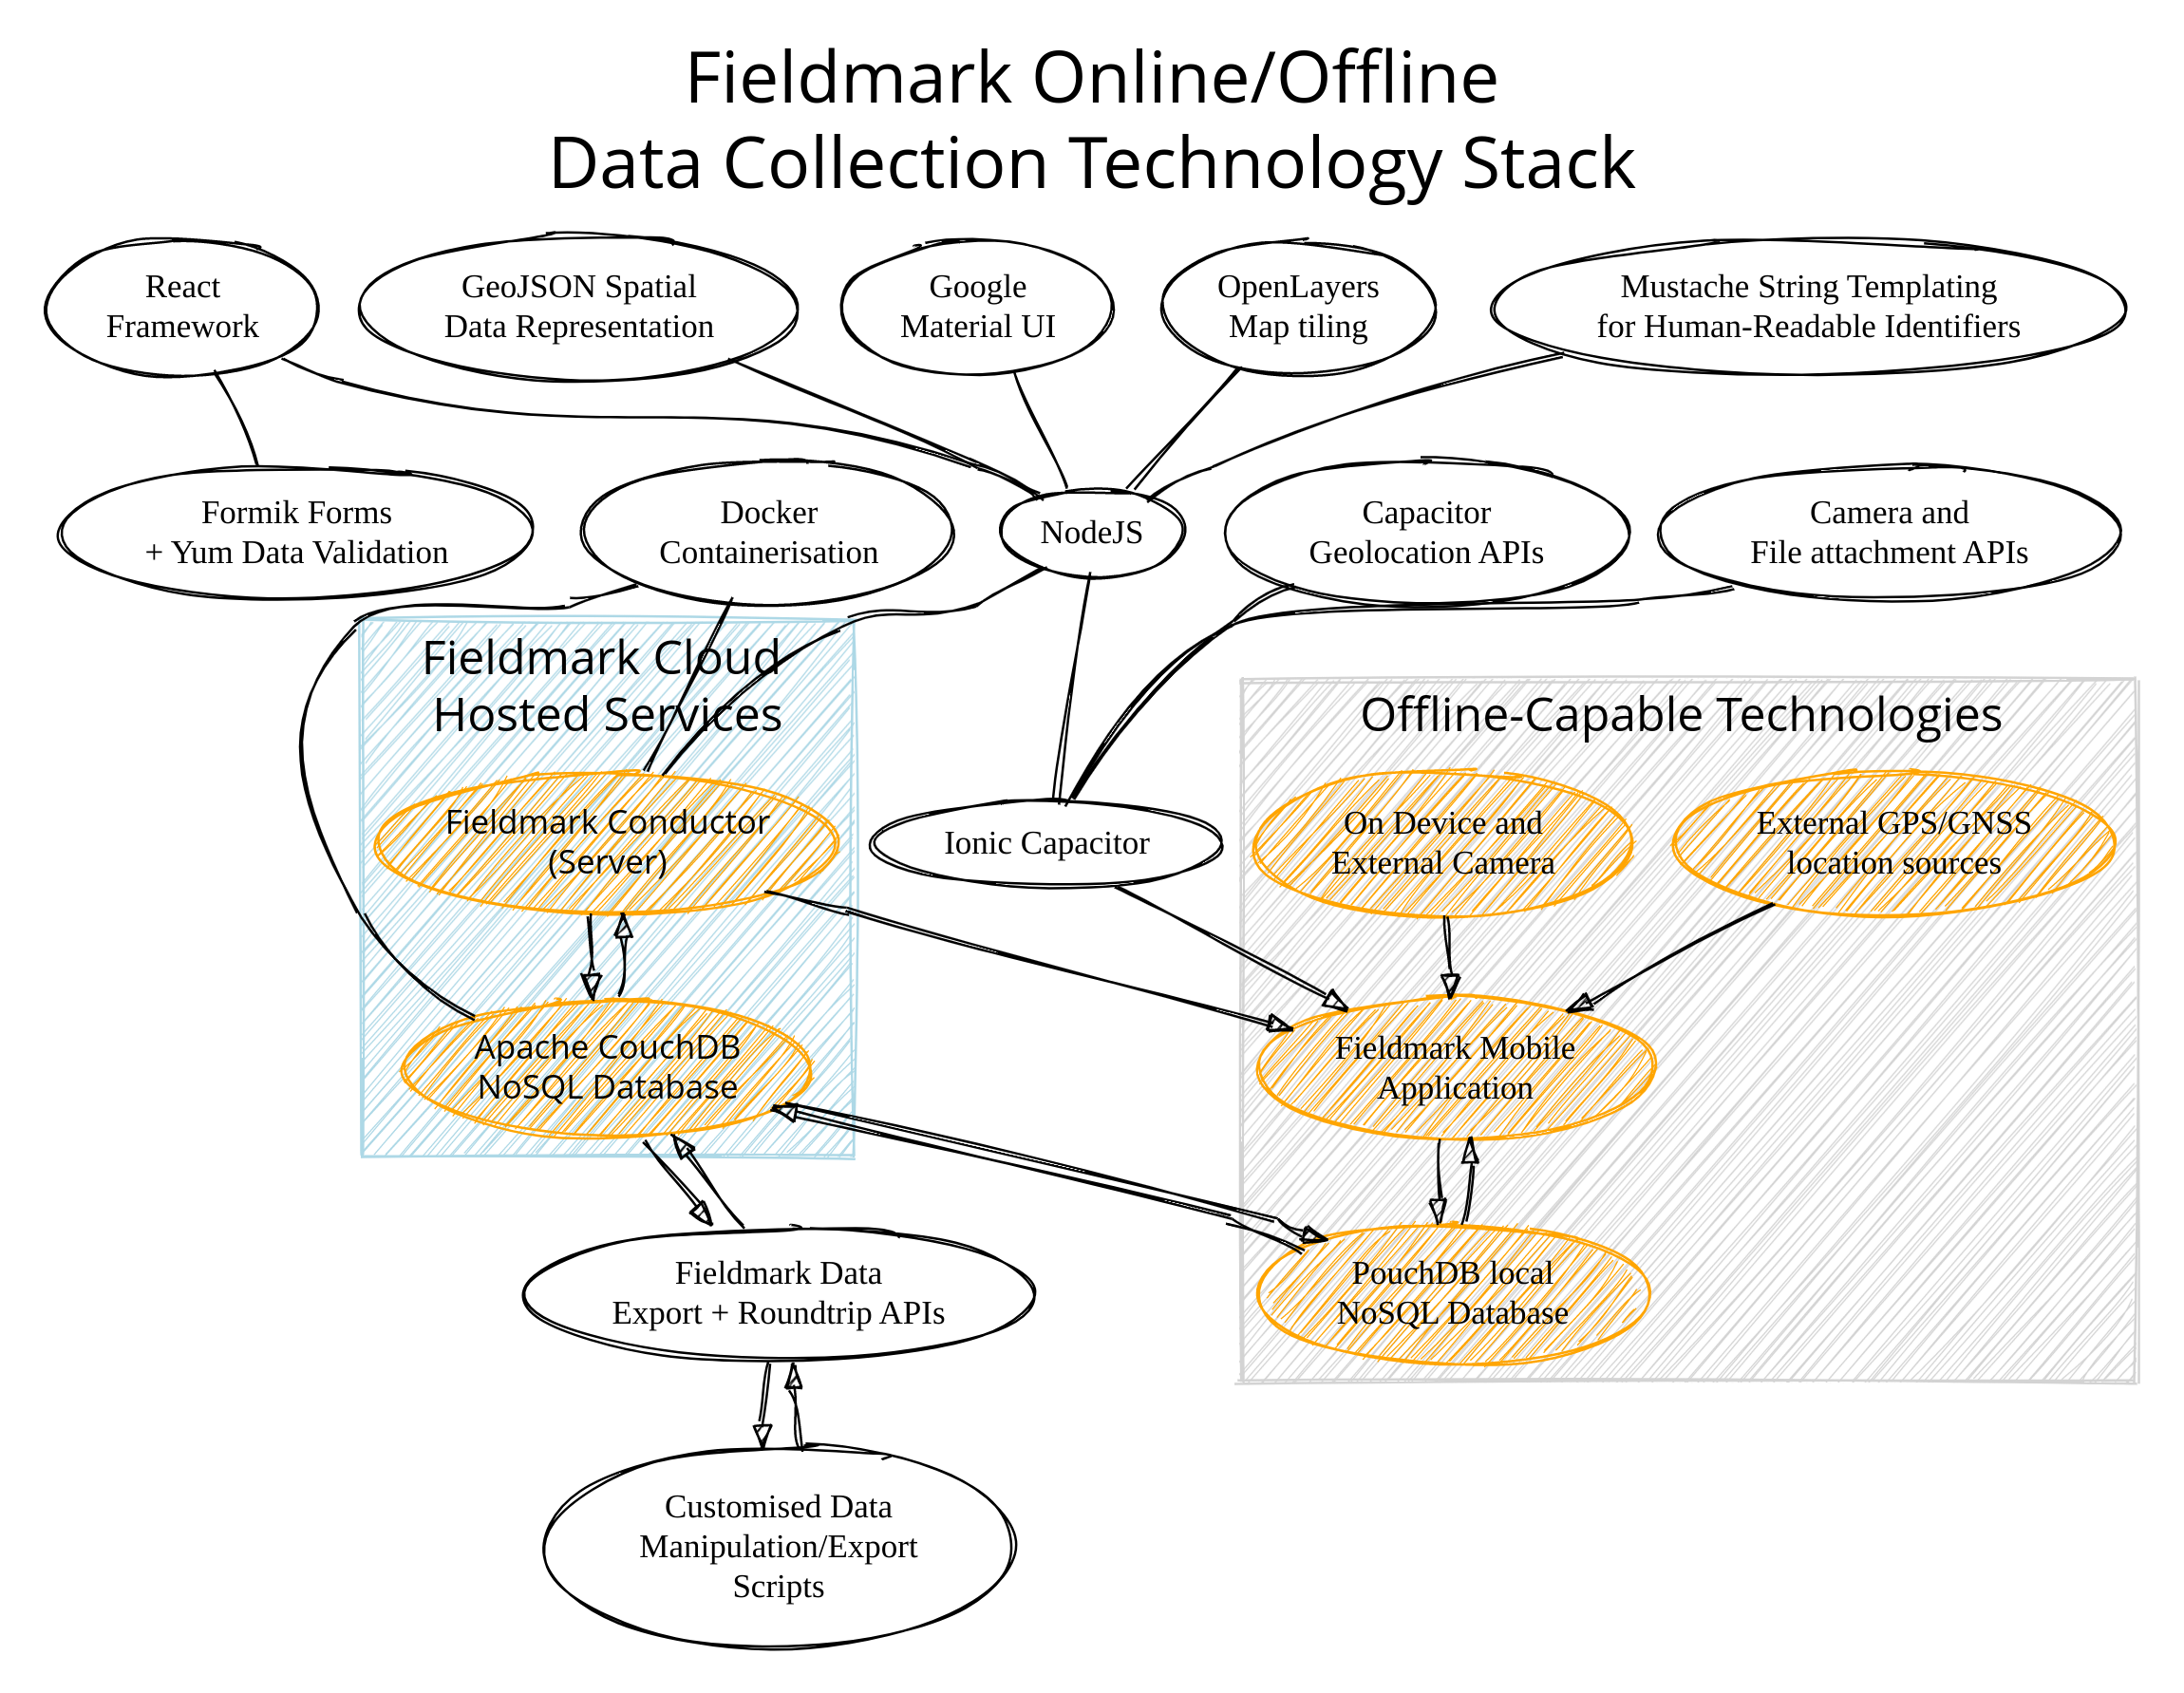
\includegraphics[width=\textwidth]{Images/bcf-diagram2.png} 
\end{column}

\end{columns}

% Technical elaboration in 2020 produced an \href{https://zenodo.org/record/4616766}{Elaboration Report}; our approach includes:
%     \begin{itemize}
%         \item Node.JS
%         \item NoSQL datastore (Apache CouchDB / PouchDB)
%         \item APIs for data interactions (CouchDB)
%         \item Progressive JS Single Page Application wrapped in Native code
% for cross-platform support using Capacitor
%         \item JSON Forms
%         \item Javascript mapping library (OpenLayers)
%         \item Plugin architecture

%     \end{itemize}
\end{frame}
%----------------------------------------------------------------------------------------


\begin{frame}{FAIMS 3.0 development approach}
Other planned, but not yet elaborated, technical capabilities include:
    \begin{itemize}
        \item Web application to provide GUI to produce definition files
        \item `Real' user management and security
        \item Interoperability with Cloudstor, EOSC nodes, ELNs, domain repositories (data `round-trip' export-modify-import)
        \item Device support (cameras, printers, instruments, etc.)
        \item Offline mapping
        \item Audio/video management
    \end{itemize}
\end{frame}

%----------------------------------------------------------------------------------------

\begin{frame}
    \frametitle{FAIMS 3.0 development progress}
        \begin{itemize}
            \item \href{https://docs.google.com/document/d/13eTN8jhJa3Pgs9GOdo7r4jtIQcskNo7ikxJcBDBKHzw/edit}{Technical Elaboration Report} was approved in February. This established the proof-of-concept for FAIMS3. 
          \item \href{https://github.com/FAIMS/FAIMS3/releases/tag/v0.1.0-alpha}{Alpha prototype} was released on 11 June 2021. 
          \item Beta prototype was released on 2 December 2022.
       %   \item FAIMS3 Beta development commenced on 5 July 2021 and  concluded 2 December 2022. 
        \item CSIRO supported extra development January -- July 2022.
         %   \item Alpha prototype passed \href{https://doi.org/10.5281/zenodo.5030772}{user-acceptance testing} on 15 June 2021.
        \item FAIMS3 code has been licensed under the \href{https://www.apache.org/licenses/LICENSE-2.0}{Apache2} license, a Developer Contribution agreement is being applied to all code affirming the license. 
        \item The FAIMS3 repository is now public on \href{https://github.com/FAIMS/FAIMS3}{GitHub}.

  \end{itemize}



\end{frame} 